\section{Experiments}

\subsection{Real datasets}
In order to test our implementation, we used three datasets of polygons.  The first one is the California Census Tracts - CCT. The layer A collects the census tracts in California during 2000 meanwhile the layers B collects those ones for 2010.  Something to note with this dataset is that the differences between the layers no just show the changes in time but also they present a small spatial gap (due to technical reasons) between the polygons which will increase considerably the number of intersections and new faces the DCEL should be able to identify.

The second dataset is the complete Census Tracts dataset for all the states of the Union in mainland.  It was collected from the official website of the United States Census Bureau\footnote{\url{https://www2.census.gov/geo/tiger/TIGER2010/TRACT/}}.  The data was clipped to select just the states inside the continent to keep the study area as compact as possible and remove some territories that does not have complete data. The layers correspond to years 2000 and 2010. The two layers are quite similar although they also present a spatial gap similar than the CCT dataset.  The CCT dataset is a subset of this dataset just for the state of California.

The third dataset is from the Global Administration Areas - GADM\footnote{\url{https://gadm.org/}}. It collects geographical boundaries of the countries and their administrative divisions around the globe.  For the tests, we select the levels 2 (States) and level 3 (Counties).  However no all the countries show administrative level for counties, for that reason both layers shows similar number of polygons and edges. We take individual polygons, it is, any multi-polygon was divided and each polygon was manage independently. The details of the real datasets are summarized in table \ref{tab:datasets}.  Experiments runs on a cluster of 12 nodes running Apache Spark 2.4.  Each node has 9 cores and 12G memory available.

\begin{table}[!ht]
    \caption{Datasets details.}
    \label{tab:datasets}
    \begin{tabular}{c c c c}
        \toprule
        Dataset & Layer & Number        & Number    \\
                &       & of polygons   & of edges  \\
        \midrule
        CCT   & Polygons for 2000 & 7028 & 2711639  \\
              & Polygons for 2010 & 8047 & 2917450 \\
        MainUS& Polygons for 2000 & 64983 & 35417146  \\
              & Polygons for 2010 & 72521 & 36764043 \\
        GADM  & Polygons for Level 0 & 116995 & 32789444 \\
              & Polygons for Level 1 & 117891 & 37690256 \\
        \bottomrule
    \end{tabular}
\end{table}

\subsection{CCT dataset}

The first set of experiments aim to compare the performance of the SDCEL implementation over the CCT Dataset varying the number of partitions used to divide the data. It sets the parameters of the quadtree used to split the data to obtains different values from coarse (100) to fine (15K) number of partitions (left part in figure \ref{fig:ca}).  Clearly there are a trade-off in this case.  The more partitions, each subdivision will have to deal with a smaller number of edges will means a faster execution.  However, if the number of partitions is too high, the cost to divide and collect the results will have an impact.  We can see that an optimal value can be reached around 7K partitions.  A zoom of this part of the plot is shown in figure \ref{fig:ca}.

In addition with the partition analysis, we compare the performance of the SDCEL implementation against the sequential solution offered by the CGAL library.  The independent column in the right of figure \ref{fig:ca} shows its execution time.  Clearly, the appropriate setting for the number of partitions of SDCEL can beat the sequential implementation by several orders of magnitude.

\begin{figure}[!ht]
    \centering
    \subfloat[SDCEL vs CGAL. \label{fig:ca_a}]{%
        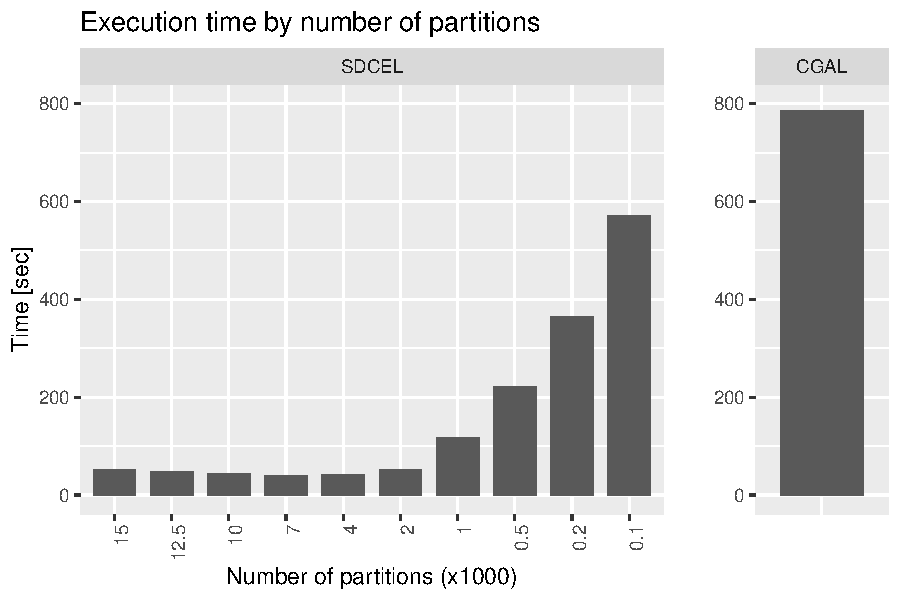
\includegraphics[width=0.9\linewidth]{figures/experiments/CA/CA.pdf}
    } \\
    \subfloat[Focus on the most relevant number of partitions. \label{fig:ca_b}]{%
        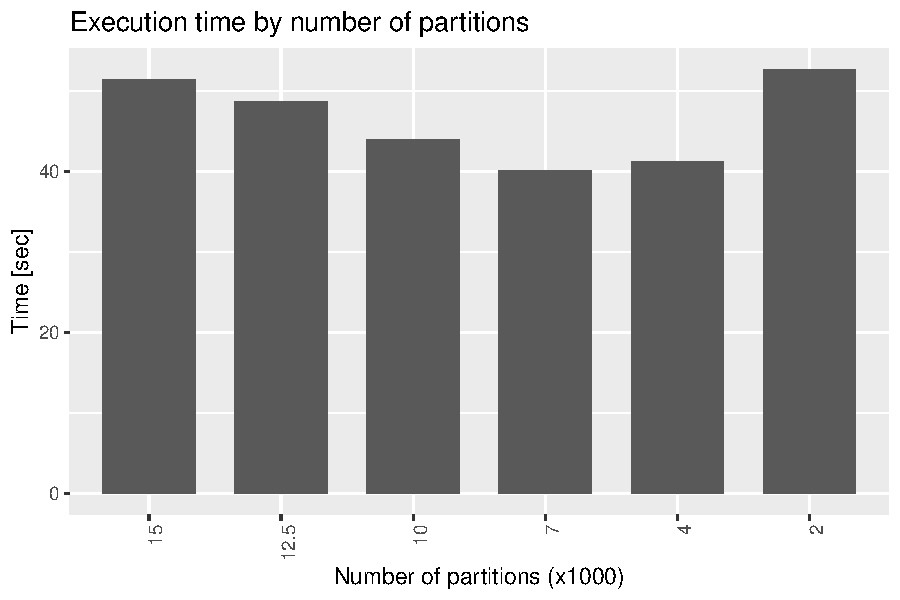
\includegraphics[width=0.9\linewidth]{figures/experiments/CA/CA_sample.pdf}
    }
    \caption{Experiments with CCTAL dataset.} \label{fig:ca}
    \Description[Experiments with the CCTAL dataset]{This figure shows the experiments using the CCTAL dataset.}
\end{figure}

\subsection{MainUS and GADM datasets}

\begin{figure}[!ht]
    \centering
    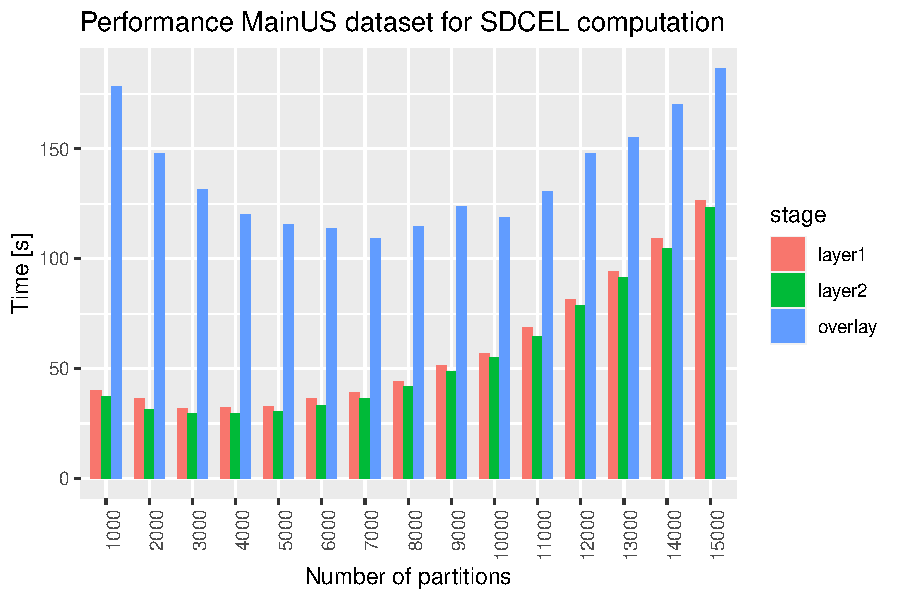
\includegraphics[width=\linewidth]{figures/experiments/MainUS/MainUS.pdf}
    \caption{Performance with MainUS dataset.} \label{fig:mainus}
    \Description[Experiments with the MainUS dataset]{This figure shows the experiments using the MainUS dataset.}
\end{figure}

\begin{figure}[!ht]
    \centering
    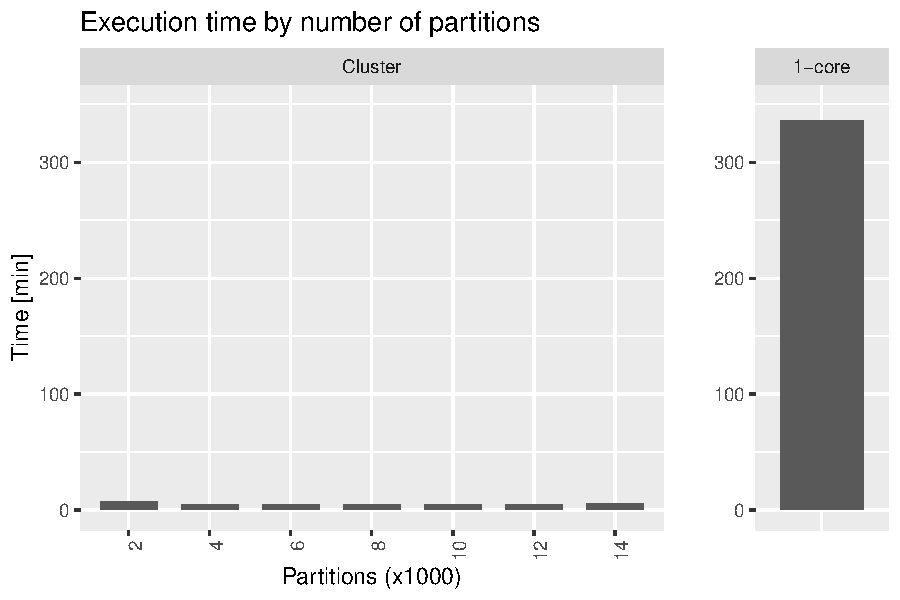
\includegraphics[width=\linewidth]{figures/experiments/GADM/GADM.pdf}
    \caption{Performance with GADM dataset.} \label{fig:gadm}
    \Description[Experiments with the GADM dataset]{This figure shows the experiments using the GADM dataset.}
\end{figure}

The CCT dataset is relatively small but useful in order to compare with the sequential alternative.  However, the CGAL library is unable to deal with big spatial data.  For MainUS and GADM datasets, we only present the results for SDCEL given that CGAL crashes when run this volume of data.  Figure \ref{fig:mainus} show the execution time of SDCEL varying the number of partitions and breaking down the execution time by stages.  Here, the time shows the performance to create the individual DCELs for each of the layers (labeled as layer1 and layer2) in addition to the time for the overlay of the two individual DCELs.  We can seen a similar trade-off as with CCT dataset in each of the stages.  We can identify a optimal number of partitions around the 6K -8K partitions.  

Figure \ref{fig:gadm} shows a similar experiment over the GADM dataset.  It plots the execution time for the SDCEL construction also divided by stages. We could identify a peak performance using between 12K and 16K partitions.  The characteristics of this dataset make it more sensible during the construction of individual DCELs particularly for the second layers which have more small polygons concentrated in some areas.

\subsection{Testing overlay alternatives}
In this section we evaluate the methods described in section \ref{sec:alternative_methods}.  We used the top 8 states from the MainUS dataset to evaluated the alternatives.  It measures the execution time of the overlay at the master/root node (`At master/root' tag), performing partitions by segment's label (`By label' tag) and performing an intermediate step at a given level (`At level [X]' tag, where X is the level given by the user).  Figure \ref{fig:overlay_tester} shows the results of the testing.  It clearly shows that the overlay by label partitions gives the best results in all the tests.

\begin{figure}[!ht]
    \centering
    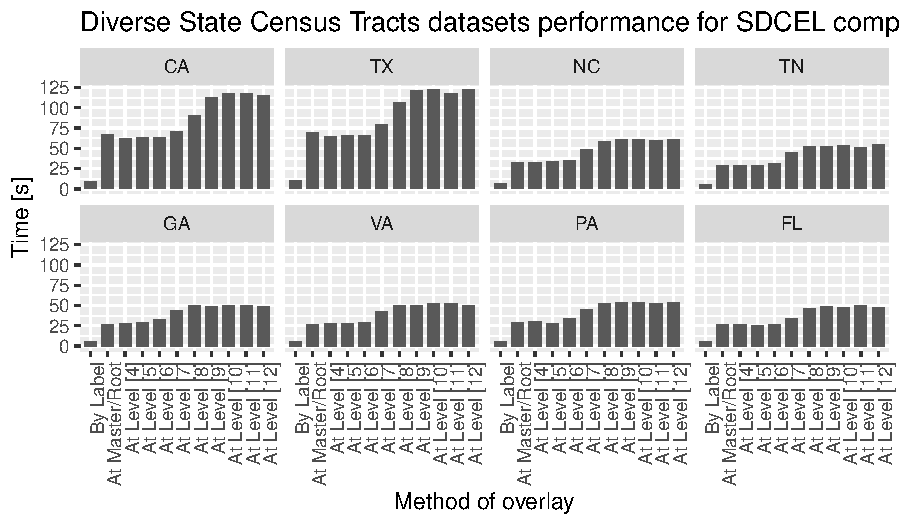
\includegraphics[width=\linewidth]{figures/experiments/Overlay_Tester/Overlay_Tester}
    \caption{Overlay methods evaluation.}\label{fig:overlay_tester}
    \Description[Overlay methods evaluation]{This figure shows the overlay methods evaluation.}
\end{figure}


\subsection{Speed up and scale up analysis}

Finally we analyze the scalability of the implementation through the speed up and scale up tests.  For the speed up, the GADM dataset was used with different amount of resources, in this case the number of available nodes.  Each time, the nodes were duplicated and the performance was measured.  Figure \ref{fig:gadm_speedup} shows  how as resources double, the response time is almost cut in half each time, as it is expected.

In the case of the scale up test, the workload was also modified.  The GADM dataset was split in 4 regions slightly similar in the number of edges they contain.  At each iteration, both the size of the data and the amount of available resources were doubled. As it was expected, the performance at each scenario should not change significantly as it is shown in figure \ref{fig:gadm_scaleup}.

\begin{figure}[!ht]
    \centering
    \subfloat[MainUS Speed Up \label{fig:mainus_speedup}]{%
        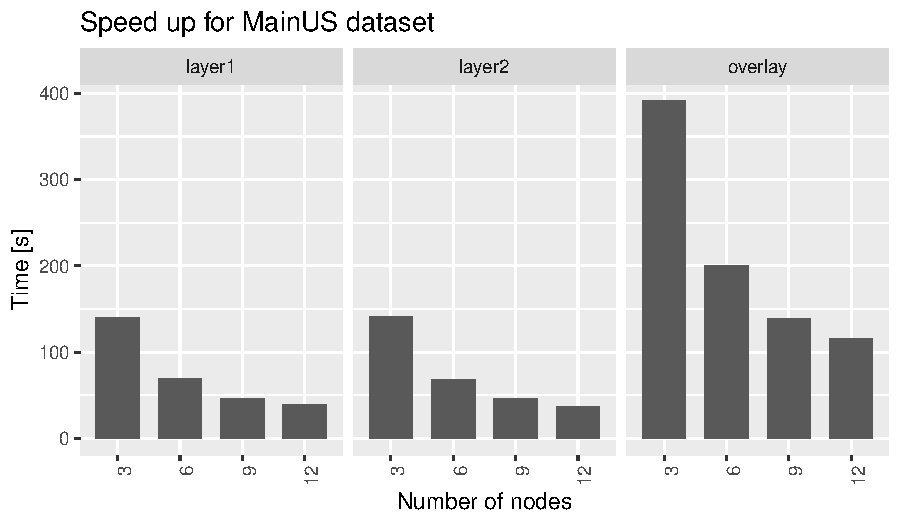
\includegraphics[width=0.9\linewidth]{figures/experiments/MainUS_speedup/MainUS_speedup}
    } \\
    \subfloat[MainUS Scale Up \label{fig:mainus_scaleup}]{%
        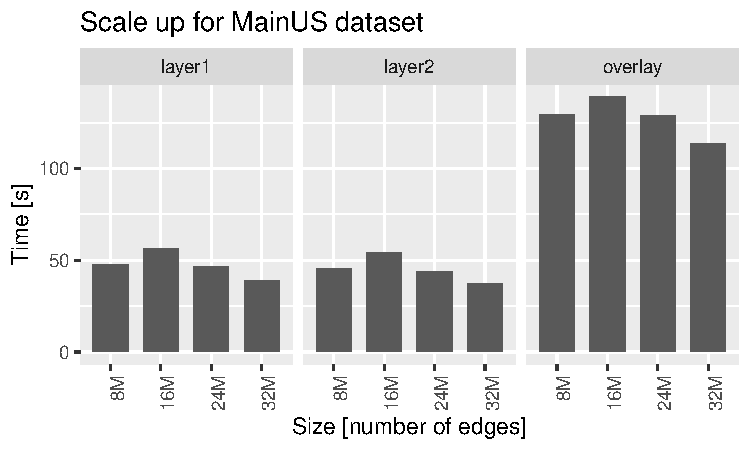
\includegraphics[width=0.9\linewidth]{figures/experiments/MainUS_scaleup/MainUS_scaleup}
    }
    \caption{Speed Up and Scale Up experiments for MainUS dataset.} \label{fig:mainus_speed_scale}
    \Description[MainUS Speed Up and Scale Up experiments.]{This figure shows the experiments for speed up and scale up analysis for the MainUS dataset.}
\end{figure}

\begin{figure}[!ht]
    \centering
    \subfloat[GADM Speed Up \label{fig:gadm_speedup}]{%
        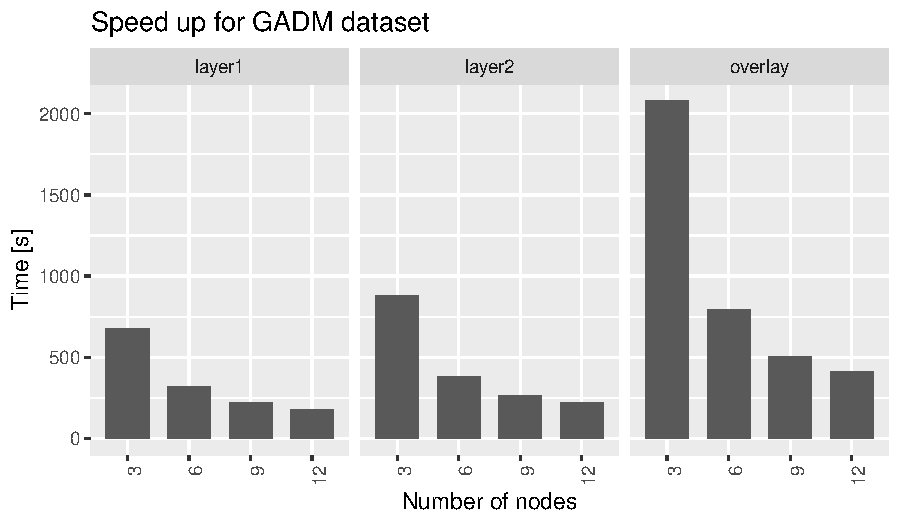
\includegraphics[width=0.9\linewidth]{figures/experiments/GADM_speedup/GADM_speedup}
    } \\
    \subfloat[GADM Scale Up \label{fig:gadm_scaleup}]{%
        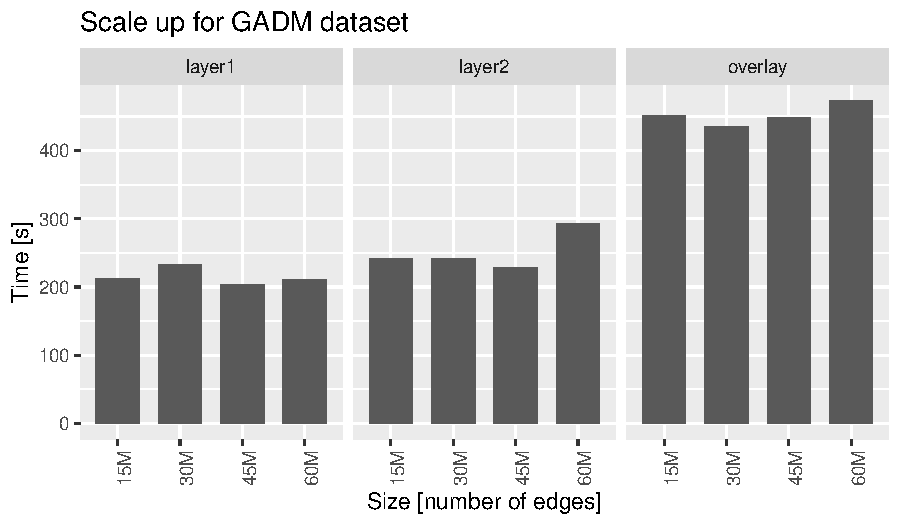
\includegraphics[width=0.9\linewidth]{figures/experiments/GADM_scaleup/GADM_scaleup}
    }
    \caption{Speed Up and Scale Up experiments for GADM dataset.} \label{fig:gadm_speed_scale}
    \Description[GADM Speed Up and Scale Up experiments.]{This figure shows the experiments for speed up and scale up analysis for GADM dataset.}
\end{figure}

\subsection{Unbalance cell analysis}

This section discusses the experiments and evaluation of the method of filter by sweep proposed in section \ref{sec:unbalance}. Figure \ref{fig:unbalance_tester1} shows the behaviour of the two methods (filter by sweep and traditional) under controlled data.  Edges from the state of Pennsylvania where taken increasing from one of the layers adding 3K edges each time and then an overlay over another layer of 3K was performed.  It simulates the actions inside an individual cell when an unbalanced number of edges for each layer must to be evaluated. It can be seen that once the data from the involved layers show increasingly unbalanced amount of data (that is, much more edges from one of the layers than the other) the filter by sweep method overcomes the traditional one on those cells with this kind of data.

\begin{figure}
    \centering
    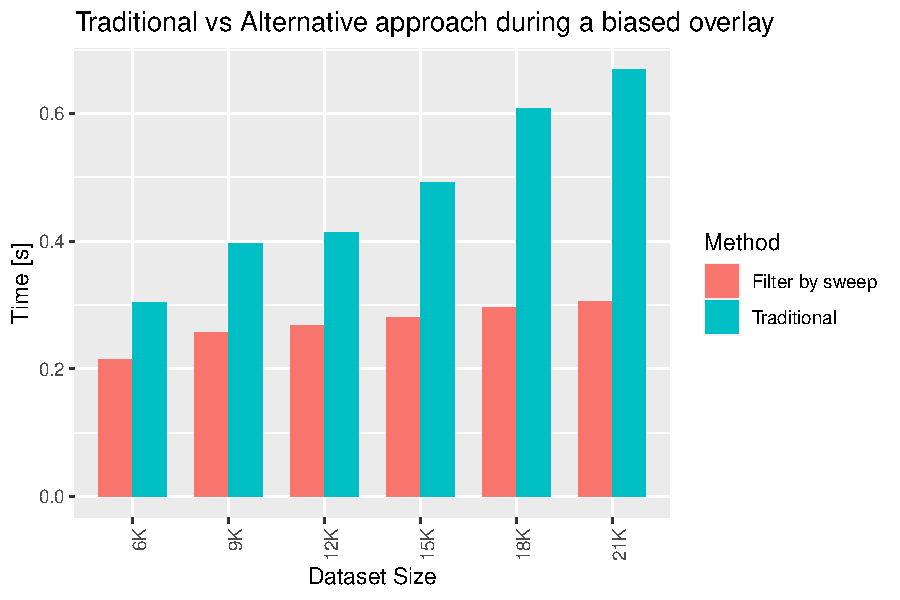
\includegraphics[width=\linewidth]{figures/experiments/Unbalance_Tester/Unbalance_Tester01.pdf}
    \caption{Unbalance cell methods evaluation.}\label{fig:unbalance_tester1}
    \Description[Unbalance cell methods evaluation]{This figure shows the Unbalance cell methods evaluation.}
\end{figure}

In addition, figure \ref{fig:unbalance_tester2} shows a similar scenario, this time using real data from the construction of the overlay DCEL of GADM dataset. For this experiment, a number of 10 cells were chosen with different percentage of disparity. It means that a 0.1 (10\%) difference happens when a layers is 10\% bigger than the other one. An average of the 10 cells for each case is shown in the figure and it compares the traditional method and the filter by sweep alternative.  Similar than in the previous case, it can be seen that the proposed method works better in cases where the number of edges for each layer is significant.

\begin{figure}
    \centering
    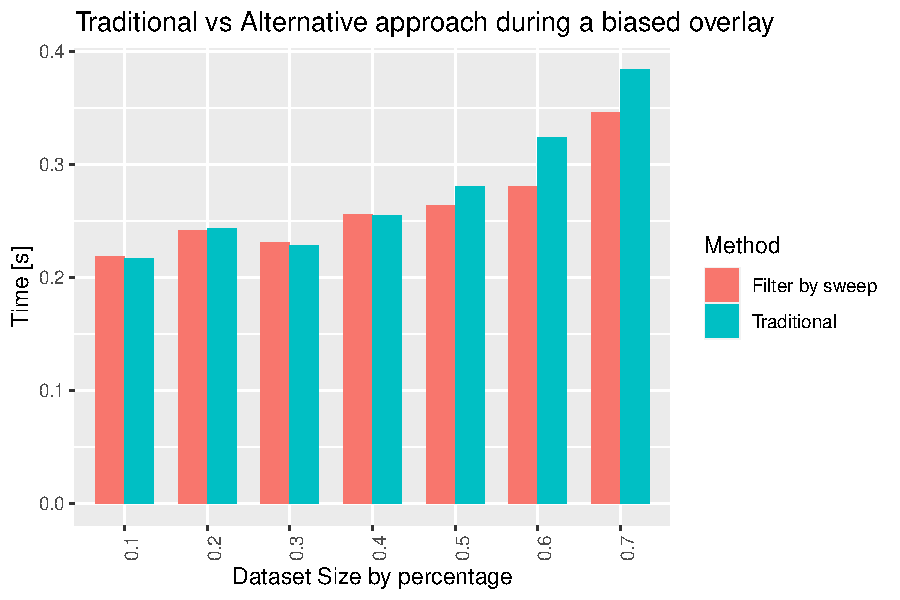
\includegraphics[width=\linewidth]{figures/experiments/Unbalance_Tester/Unbalance_Tester02.pdf}
    \caption{Unbalance cell methods evaluation.}\label{fig:unbalance_tester2}
    \Description[Unbalance cell methods evaluation]{This figure shows the Unbalance cell methods evaluation.}
\end{figure}